
%\chapter{Une nouvelle approche pour prédire le type de transition dans le phénomène de percolation}   
\chapter{Percolation dans les réseaux complexes}
\begin{minipage}{\textwidth}
	\linespread{1.2}
	\minitoc
\end{minipage}

\newcommand{\kma}{\textless k_a \textgreater}
\newcommand{\kmap}{\textless k'_a \textgreater}
\newcommand{\kmaa}{\textless k_a^2 \textgreater}

\section{Introduction}
%La détermination du type de transition de phase dans le phénomène de percolation n'est pas encore devenue une science exacte, car on manque d'une règle qui  peut déterminer, a priori, quelle transition sera de premier ou de second ordre. Cependant la détermination se fait juste après la transition, l'objective de ce chapitre est d'apporter une contribution concernant ce problème qui est un sujet très important au point de vue de la physique fondamentale.\\
%Le but ultime de l'étude des réseaux est de mieux comprendre le comportement des réseaux des systèmes. Par exemple, nous étudions la structure d'Internet pour mieux comprendre la manière avec laquelle le trafic Internet  circule, la façon du fonctionnement des protocoles de communication, ou comment organiser le réseau afin de le rendre plus performant, nous étudions les réseaux biochimiques comme les réseaux métaboliques car nous espérons qu'ils permettent de    comprendre les processus chimiques complexes qui se déroulent dans la cellule, ou des outils algorithmiques pouvant nous aider à obtenir des informations biologiques de grands volumes de données générées \cite{Newman2010}, nous étudions le réseau causal qui représente la structure à grande échelle de l'espace-temps dans notre univers accéléré, pour comprendre pourquoi ce réseau est aussi un graphe de loi sans-échelle avec un regroupement fort \cite{Sungryong-Arjun2015}.\\
%Alors le but, à part le rappel théorique, est de mieux comprendre le comportement des transitions de phase dans les réseaux réels à partir
%des approches dans le domaine des réseaux complexes. En bref, nous allons établir une formule pour prévoir le type de transition de phase au voisinage du point critique.

%\section{Transition de phase}
Comme dans la fusion de la glace, le ferro-magnétisme, la supraconductivité et le repliement des protéines, la nature manifeste quotidiennement des transitions de phase: processus dans lesquels les systèmes changent radicalement certaines propriétés physiques lorsqu'une variation minimale des variables se produisent.\\
La grande présence des transitions de phase dans le monde réel a poussé les physiciens, depuis le tout début de la mécanique statistique, à découvrir des comportements universels et critiques ainsi que de faire un grand effort pour la classification de ces transitions de phases. La première tentative à fournir une classification a été réalisée par Ehrenfest \cite{Ehrenfest1933}.  Actuellement, les schémas de classification les plus modernes regroupent les transitions de phase en deux grandes catégories : de premier et de second ordre.\\
En thermodynamique, les transitions de phase du premier ordre sont celles qui impliquent une chaleur latente, c'est-à-dire au cours d'elles le système absorbe ou libère une quantité typiquement élevée d'énergie par volume. Normalement, elles sont caractérisées (au point de transition) par "un régime en phase mixte", dans lequel certaines parties du système ont subi la transition et d'autres non, en présence ainsi d'une sorte de coexistence des phases des deux régimes. Les signes de telle transition sont: le comportement abrupt et discontinu du paramètre d'ordre à proximité du point de transition, ainsi que l'irréversibilité intrinsèque de la transition, avec la présence (dans la majorité des cas) de boucles hystérésis. Par contre, les transitions de phase de second ordre (également appelées transitions de phase continues) sont réversibles et correspondent à des paramètres d'ordre présentant un comportement continu au voisinage du point de transition.
Parmi les transitions du premier ordre nous citons la fusion de la glace, l'ébullition de l'eau, et les transitions de super-refroidissement et de surchauffe. Pour le second ordre nous avons la transition ferromagnétique, la supraconductivité et la transition super-fluide.
\section{Percolation}
La percolation est l'émergence d'une connectivité à grande échelle. L'ampleur de la connectivité qui apparaît soudainement à un point de transition a un impact profond sur les comportements macroscopiques d'un système.\\
Le terme de percolation a  été introduit pour la première fois  en $1956$ par Broadbent et Hammersley \cite{Broadbent-Hammersley1957}, lors  de leur étude de l'écoulement d'un fluide  dans  un milieu poreux. La théorie développée depuis lors , dite de la percolation, s'appuie sur des considérations statistiques pour caractériser le comportement d'un ensemble d'objets incomplètement connectés. Dans un  tel système, la communication à longue distance est soit possible soit impossible selon le nombre d'objets et de contacts entre eux. La transition entre ces deux régimes est repérée par le point où  le paramètre décrivant la connectivité prend une valeur critique, qu'on appel le seuil  de percolation. Ainsi, on passe d'un  état de connectivité à courte distance à un état de connectivité à longue distance lorsqu'on franchit cette valeur seuil, en faisant croître continûment la concentration des objets et/ou de leurs liens. Les propriétés du système changent alors brusquement en ce point, et  la transition de percolation se comporte comme une transition de phase du deuxième ordre (ou continue). Cette théorie, qui est désormais entrée dans lé cadre connu des transitions de phases, s'est fortement développée au cours des dernières décennies, compte tenu  du nombre croissant de  ses domaines d'applications. On peut par exemple citer les transitions para-ferromagnétique dans les alliages magnétiques dilués, états localisés-états étendus dans les semi-conducteurs amorphes, sol-gel dans les polymères, métal-supraconducteur ou isolant-conducteur dans les composites \cite{Stauffer1982}. Actuellement, la percolation est également au centre des investigations sur les réseaux sociaux, biologiques, et artificles \cite{Newman-al2002,Dorogovtsev-al2008,Rozenfeld-al2010}.\\
Un processus de percolation standard peut avoir lieu, en général, par deux types: par sites ou par liens. La percolation par sites sur un graphe donné signifie que les sommets sont vides avec une probabilité donnée $p$ (ou occupée avec une probabilité $1-p$), tandis que la percolation par liens fait référence à l’existence ou non d’un bord entre deux nœuds choisis arbitrairement. Une fois la suppression (ou le placement) aléatoire des nœuds ou des arêtes effectuée, plusieurs quantités permettent la caractérisation des propriétés du réseau.
On examine généralement l’existence et la taille de l'amas infini, appelée aussi composante géante, en fonction $p$, ainsi que la taille moyenne et les fluctuations de la taille des amas finis (ou petites composantes). De cette manière, on définit une probabilité critique $p_c$ en dessous de laquelle le réseau percole, et un ensemble d’exposants critiques caractérisant la transition de phase (Fig.~\ref{percolation}).

\begin{figure}[h!]
	\centering
	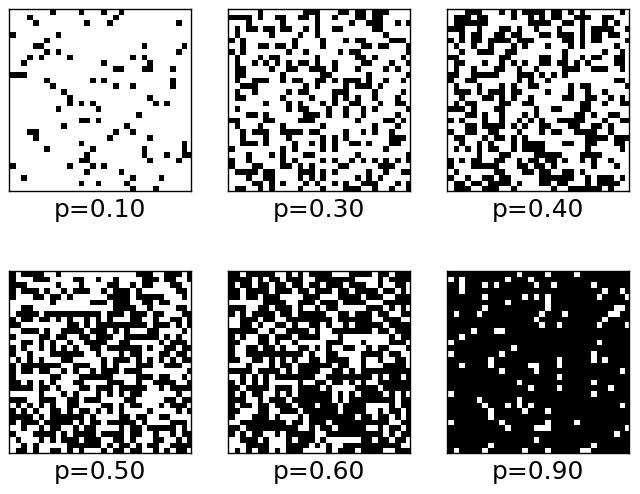
\includegraphics[scale=0.5]{./figures/percolation}
	\caption{Une démonstration de percolation par site sur une grille à deux dimensions pour différentes valeurs de $p$. Sous le seuil de percolation le système est composé de petits amas, après un certain point critique $p_c$ un amas ``infini`` occupe la grille.}
	\label{percolation}
\end{figure}

%Dans la percolation par liens, on commence par $n$ nœuds non connectés. A chaque pas de temps, un lien est ajouté entre deux nœuds sélectionnés selon une règle donnée. Le nombre de liens $E$ ajouté à un certain pas de temps divisé par la taille du système est le paramètre de contrôle $\km=\frac{2E}{n}$ qui décrit la transition de phase. En ce qui concerne le paramètre d'ordre, on peut prendre la fraction de nœuds appartenant à la composante géante du réseau (généralement noté $S(t)$). Au fur et à mesure que le temps augmente, le nombre de liens ajoutés dans le réseau augmente, dans la limite thermodynamique ($N\longrightarrow \infty$), $S(t)$ présente une transition de phase de zéro à $O(1)$ au voisinage d'un point critique ($\km_c$). 
\subsection{Percolation dans le réseau aléatoire d'Erd\H{o}s-Rényi}
Un réseau aléatoire peut être créé en spécifiant que chaque paire de nœuds est connecté par un lien avec une probabilité uniforme $p$. Ce type de réseaux a été étudié d'un point de vue mathématique pure par Erd\H{o}s et Rényi \cite{Erdos-Renyi1959,Erdos-Renyi1960,Erdos-Renyi1961}, il est souvent désigné par son nom mathématique $G(n,E)$, avec $n$ est le nombre de nœuds et $E$ le nombre de liens. 
Dans la cas où $n$ est très grand, plusieurs propriétés de l'ensemble des réseaux aléatoires ont été exprimées analytiquement et parfois exactement.\\
Les réseaux aléatoires ER sont les plus étudiés parmi les modèles de réseaux, leurs propriétés structurelles varient en fonction de $p$ montrant notamment un changement radical à une probabilité critique $p_c=\frac{1}{n}$,
correspondant à un degré moyen critique $\textless k \textgreater_c=1$. Erdös et Rényi ont prouvé que:\\
\begin{itemize}
	\item Si $p <p_c$, lorsque $n$ tend vers l'infini, le réseau n'a quasiment pas de composante de taille  
	supérieure à $(\ln(n))$.
	\item Si $p=p_c$, la composante la plus importante a quasiment la taille de $n^{\frac{2}{3}}$.
	\item Si $p> p_c$, le réseau a une composante de taille de l'ordre de $n$ et aucune autre composante n'a de taille supérieure à $(\ln(n))$.
\end{itemize}
\begin{figure}[h!]
	\centering
	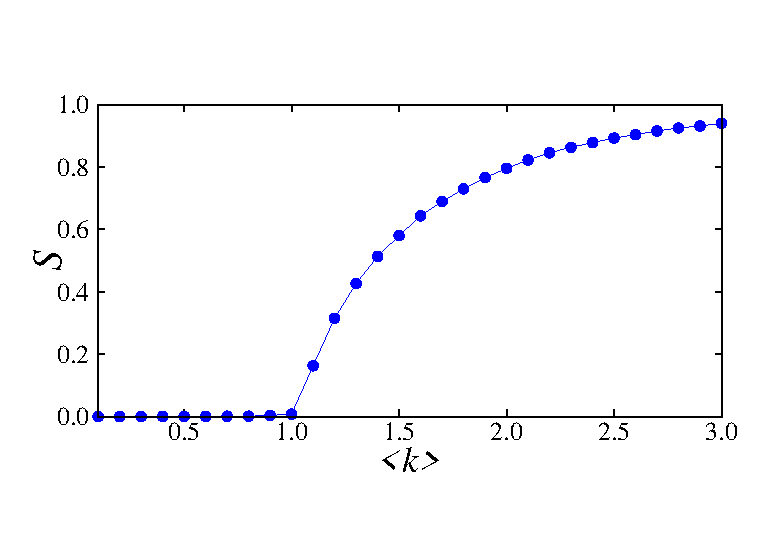
\includegraphics[width=12cm,height=9cm]{./figures/fig-ER-CG}
	\caption{Les simulations numériques du seuil de percolation dans le modèle ER en fonction du degré moyen, pour un réseau de taille $n=10^5$. On observe que le point où la fraction de la composante géante, $S$, émerge est à $\textless k\textgreater=1$.}
	
	\label{percolation-graph}
\end{figure}

La transition au $p_c$ présente les caractéristiques typiques d'une transition de phase de deuxième ordre (voir Fig.~\ref{percolation-graph}). En particulier, si on considère la fraction de noeuds appartenant à la composante la plus importante comme paramètre d'ordre, la transition tombe dans la même classe d'universalité que celle des transitions de percolation de champ moyen. Erdös et Rényi ont étudié la distribution des degrés minimum et maximum dans le graphe aléatoire, mais la distribution des degrés complète a été obtenue plus tard par Bollobás \cite{Bollobas1998}. La probabilité qu'un nœud ait un degré $k$ suit la distribution binomiale:
\begin{equation}
P(k)=C^k_{n-1}p^k(1-p)^{n-1-k}.
\end{equation}
Pour $n$ très grand,  cette distribution devient une distribution de Poisson:
\begin{equation}
P(k)=e^{-\textless k\textgreater}\dfrac{\textless k\textgreater^k}{k!}.
\label{ER}
\end{equation}
\begin{figure}[h!]
	\centering
	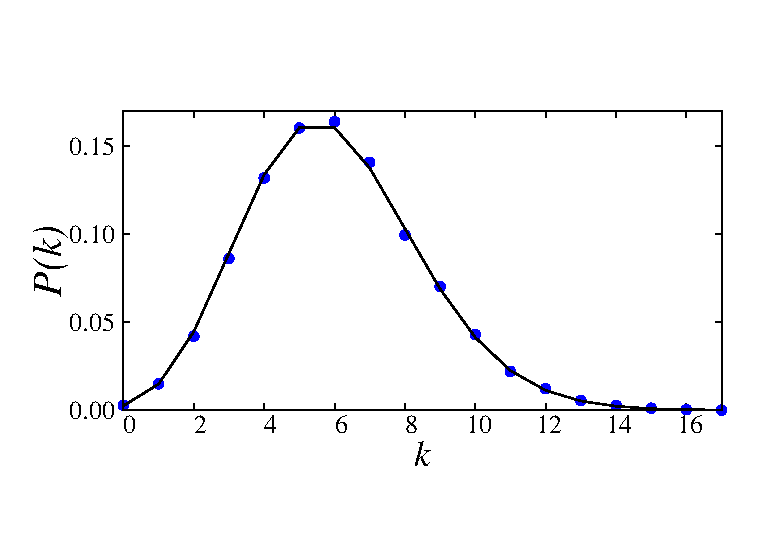
\includegraphics[scale=1]{./figures/fig-ER-dist}
	\caption{Distribution des degrés d'un réseau aléatoire ER de degré moyen $\km=6$, les cercles représentent les simulations numériques et la ligne noire représente l'Eq.~\eqref{ER}.}
	
	\label{ER-distribution}
\end{figure} 

Le coefficient de clustering, $C$, est une quantité très simple à calculer pour le graphe aléatoire, rappelons qu'il est défini comme la probabilité que deux voisins d'un nœud du réseau soient également voisins les uns des autres. Dans un graphe aléatoire, la probabilité que les deux nœuds soient voisins est égale à $p=\frac{\textless k\textgreater}{(n - 1)}$. Par conséquent:

\begin{equation}
C=\dfrac{\textless k\textgreater}{(n - 1)}
\end{equation}

Cette valeur de $C$ qui tend vers $0$ quand $n$ tend vers l'infini est l'un des nombreux aspects dans lesquels le graphe aléatoire diffère fortement de la plupart des réseaux réels, dont beaucoup ont des coefficients de clustering assez élevés.

\subsection{Percolation explosive}
Une idée prévalente, pendant assez de temps, est que la plupart des transitions de la percolation classique (ordinaire) semblent être de second ordre (continue) comme la percolation par liens dans les réseaux ER. Dans ce cas,  la taille de la composante géante augmente progressivement lorsque le paramètre de contrôle qui est le degré moyen $\km$ dépasse le seuil de percolation. Il convient toutefois de noter qu'il existe également des exemples, bien que rares, de modèles de percolation présentant une transition de phase de premier ordre (discontinue), tels que les percolations bootstrap \cite{Adler1991}, k-core \cite{Dorogovtsev2-2006}, et brouillage \cite{Echenique-al2005}.\\ 
Les transitions de phase de percolation de premier ordre ont suscité un intérêt considérable depuis le travail de Achlioptas et al. \cite{Achlioptas-al2009}. Dans ce travail, les auteurs fournissent des preuves solides, mais finalement trompeuses, que la connectivité à grande échelle émerge dans une transition de phase discontinue qu'ils ont appelés ''percolation explosive``.\\
La percolation explosive (PE) est un phénomène qui résulte souvent de petites interventions conçues pour retarder la transition de phase de percolation. Le déclenchement peut en effet être considérablement retardé, mais une fois la transition de percolation atteinte inévitablement, une connectivité à grande échelle apparaît de manière brusque \cite{Costa-al2010,Costa-al2015,Cho-Kahng2011}.
L'idée principale du processus Achlioptas (PA) \cite{Achlioptas-al2009} est de modifier la règle pour générer des graphes ER. Au lieu d'ajouter des liens aléatoires, dans le PA on choisit deux liens au hasard puis on utilise une règle pour sélectionner l'un ou l'autre. Le lien sélectionné sera ajouté au graphe alors que l'autre lien sera rejeté.\\ 
Dans \cite{Achlioptas-al2009}, les auteurs se sont demandés s'il était possible de déplacer le point critique de la transition de phase de percolation suivant une règle de sélection appropriée. Une règle qui peut naturellement être imaginée c'est la règle du produit: Parmi les liens donnés, choisir celui qui minimise le produit des tailles des composantes contenant les quatre extrémités de $\{e_1,e_2\}$ (voir Fig.~\ref{achlioptas}). Cette règle a été suggérée dans \cite{Bollobas-1984} comme la plus susceptible de retarder le point critique. Une autre règle est la règle de la somme, où la taille de la nouvelle composante formée est minimisée.
Considérons la Fig.~\ref{achlioptas}: (\textbf{A}) l'évolution du réseau  selon le modèle ER, à chaque étape deux nœuds sont choisis au hasard et reliés par un lien (représenté par la ligne pointillée). Dans cet exemple, deux composantes de taille $7$ et $2$ sont fusionnées. (\textbf{B}) Deux liens aléatoires $\{e_1,e_2\}$ sont sélectionnés à chaque étape mais un seul sera ajouté au réseau suivant une règle de sélection, tandis que l'autre sera abandonné.
Suivant la règle de produit (RP), le lien sélectionné est celui qui minimise le produit des tailles des composantes qui sont fusionnées. Pour cet exemple, $e_1$ (avec le produit $2\times7=14$) sera choisi et $e_2$ rejeté (parce que $4\times4=16$). En revanche, la règle avec laquelle on sélectionne le lien minimisant la somme des tailles des composantes choisi $e_2$ au lieu de $e_1$. (\textbf{C}) Évolution de la  fraction de noeud dans la composante géante  $S$ pour: ER, BF (une règle de taille bornée, voir \cite{Bohman-Frieze2001}), et RP. Le réseau étudie est de taille $n=512000$.
\begin{figure}[h!]
	\centering
	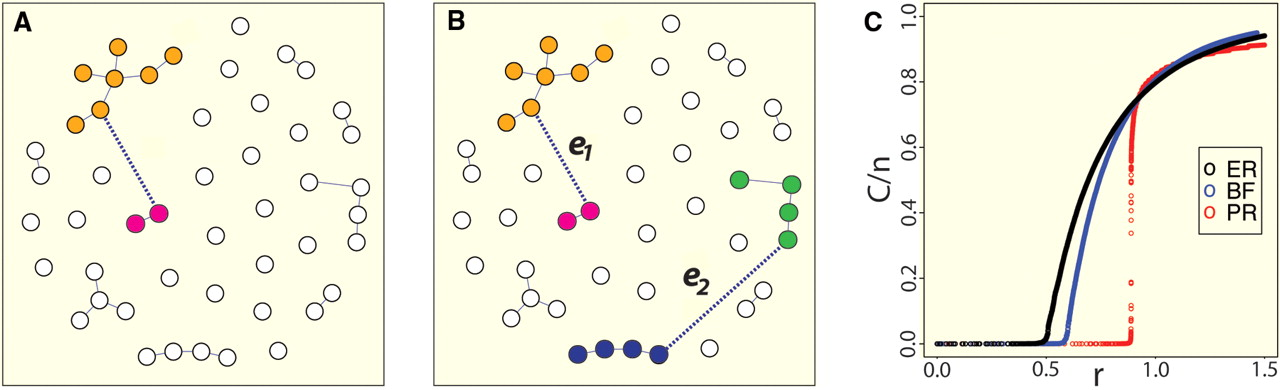
\includegraphics[scale=0.35]{./figures/achlioptas3}
	\caption{Comparaison entre la percolation aléatoire et PA. (\textbf{A}) Percolation ER classique, où les liens sont ajoutés au hasard dans le réseau. (\textbf{B}) Percolation PA, où à chaque étape deux liens sont en compétition pour être établis. (\textbf{C}) Paramètre d'ordre: la taille relative de la composante géante par rapport au nombre des liens ajoutés normalisés par la taille du système.}
	\label{achlioptas}
\end{figure}

 La Fig.~\ref{achlioptas}.(c) peut suggèrer que la transition de percolation RP est discontinue. Sur la base de l’analyse de l’intervalle de transition, il a été avancé que la transition de percolation sous AP est explosive et discontinue \cite{Achlioptas-al2009}.
 %Achlioptas et al. ont utilisé une méthode intéressante pour vérifier que la transition est bien discontinue. Ils mesurent numériquement le pas de temps $t_0$ auquel la taille de la composante géante $(C)$ devient plus grande que $n^{\frac{1}{2}}$, et $t_1$ où $C$ devient plus grand que $\frac{1}{2}\times n$. Un pas de temps correspond à une valeur de $r$ tel que $r=\frac{E}{n}=\frac{t}{n}$ (puisque le nombre de liens à l'instant $t$ est $E$). Pour le modèle ER et d'autres transitions de percolation continues, on trouve que $\Delta\equiv t_1-t_0$ est extensive, c'est-à-dire il évolue avec $n$. En outre, pour le modèle RP, ils ont trouvé que $\Delta\sim n^{\frac{2}{3}}$. Puisque $\Delta$ est sous-linéaire en $n$, c'est un argument numérique qui montre que dans la limite thermodynamique $n\rightarrow \infty$ la transition de percolation est en effet discontinue.
Cependant, cette conjecture a été rapidement et  rigoureusement désapprouvée par Riordan et Warnke \cite{Riordan-Warnke2011,Riordan-Warnke2012}, en montrant qu'il ne s'agit pas d'une transition discontinue  mais continue. En effet, leur argument montre des transitions de phase continues pour une classe encore plus grande de processus PA \cite{Riordan-Warnke2012}. Leurs résultats indiquent que la continuité de la transition de phase est une caractéristique assez robuste et donc tous les processus Achlioptas ont une transition de phase continue. En revanche, Nagler et ses collègues \cite{Nagler-al2012} ont montré qu'il est également vrai que certains processus de percolation basés sur le choix d'un nombre fixe de sommets aléatoires sont discontinus, et ils ont résolu ce paradoxe apparent. En identifiant et analysant un processus  continu dans le sens défini par Riordan et Warnke \cite{Riordan-Warnke2012} mais qui présente encore un nombre infini de sauts discontinus dans un voisinage arbitraire du point de transition: un escalier du Diable. Ils ont démontré analytiquement que la continuité à la première transition de connectivité et la discontinuité du processus de percolation sont compatibles pour certains systèmes de percolations compétitifs.\\
La PE est un problème scientifique très intéressant dans des champs de recherche plus larges que la percolation. Il détient un potentiel considérable pour faire progresser notre connaissance des transitions de phase et des phénomènes critiques. Le fait qu'une légère modification des règles de sélection classiques puisse modifier de manière significative la classe d'universalité de la transition de phase sous-jacente est impressionnant. De plus, il semble que dans des cas extrêmes, l'ordre de transition lui-même puisse également changer.

\subsection{Percolation explosive dans d'autres modèles}
Au-delà de la percolation ordinaire, de nombreux autres modèles ont été développés en se basant sur diverses contraintes concernant l'occupation des liens afin de produire la PE. Dans ce qui suit, nous examinons brièvement certains de ces modèles qui sont détaillés entre autres dans la référence \cite{Boccaletti-al2016}: 
\subsubsection{Le modèle de probabilité}
Ce modèle consiste à donner pour tout amas $i$ un poids $\delta_i$, à chaque pas de temps un lien entre une paire d'amas $(i,j)$ est occupé par une probabilité proportionnelle à $(\delta_i\delta_j)^{\alpha}$. La somme  de tous les poids est déterminée comme une constante de normalisation $w=\sum_i\sum_j(\delta_i\delta_j)^{\alpha}$, alors la probabilité pour que l'amas $i$ soit lié à un autre amas $j$ est $\frac{(\delta_i\delta_j)^{\alpha}}{w}$ \cite{Cho-al2010}.\\ Un autre exemple est celui appelé le modèle hamiltonien de la référence \cite{Moreira-al2010}, on commence par un réseau de $n$ nœuds sans aucun lien, de sorte que chaque nœud appartient initialement à un amas différent. Tout d'abord, un hamiltonien $H$ simple est défini en fonction des tailles des amas et du nombre de liens ajoutés à ces amas. Ensuite, un nouveau lien $e$ entre toute paire de nœuds non encore connectés est ajouté, avec une probabilité proportionnelle à $e^{(-\beta\Delta H_e)}$, où $\Delta H_e$ est le changement d'énergie après l'ajout d'un lien.

\subsubsection{Les modèles Hybrides}
Dans les modèles hybrides la composition des arêtes suit à la fois des règles de percolation ordinaire et des règles concurrentielles: à chaque pas de temps, un lien peut être choisi aléatoirement avec probabilité $p$, alors qu'il peut aussi être choisi suivant une règle concurrentielle donnée par la probabilité $1-p$. Par exemple, dans \cite{Bastas-al2014} la RP est utilisée, dans la référence \cite{Cao-Schwarz2012} un mélange de $k=2$ et $k=3$-core sur le réseau aléatoire et un mélange de $k=3$-core et des modèles de percolation de brouillage dans le réseau 2D sont étudiés. Les modèles hybrides ont été analysés dans des réseaux 2D \cite{Cao-Schwarz2012,Bastas-al2014} et des réseaux ER  \cite{Cao-Schwarz2012,Bastas-al2014,Fan-al2012}.
\subsubsection{Les modèles bootstrap}
Dans le cadre de la PE, certains modèles bootstrap ont été proposés \cite{Baxter-al2010}. Le processus de percolation bootstrap standard sur un réseau suppose que les sites sont actifs ou inactifs, et que l'état d'un site dépend de ses voisins. Initialement, chaque site est actif avec une probabilité $p$, et inactif avec probabilité $1-p$. Chaque site activé reste dans son état, alors que chaque site inactif peut devenir actif (et rester actif pour toujours) si ses $i$ voisins les plus proches sont actifs (avec $i=2,3,\ldots$). La procédure est poursuivie jusqu'à ce que le système atteint la configuration stable . Dans l'état final du processus, on s'intéresse à savoir s'il existe  une composante géante occupée par des sites actifs. La percolation bootstrap peut montrer des transitions continues ou discontinues, selon le type du réseau et sa dimension.
\begin{sloppypar}
	
	\section{Nouvelle approche pour prédir le type de la transition dans les systèmes percolatifs}
\end{sloppypar}
\subsection{\'{E}tat de l'art}
La prédiction du type de la transition de phase est un sujet assez compliqué, et il n'existe pas encore de formalisme théorique qui traite la question d'une façon rigoureuse. Autrement dit, il manque une règle avec laquelle on peut déterminer qu'une telle transition est de premier ou de second ordre indépendamment des mécanismes locaux d'évolution du système ou modèle étudié. Et c'est le cas aussi pour la transition de percolation qui est l'un des modèles les plus simples et les plus anciens dans la physique statistique. Cependant pour quelques modèles spécifiques, par exemple dans \cite{Cho-al2010}, une équation cinétique a été utilisée pour déterminer le type de la transition de la percolation. Dans l'évolution des réseaux ER, par exemple, l'équation différentielle est écrite à la limite thermodynamique comme:
\begin{equation}
\frac{\partial n(k_a,t)}{\partial t}=\sum_{i+j=k_a}\frac{\delta_in(i,t)}{c(t)}\frac{\delta_jn(j,t)}{c(t)}-2\frac{\delta_{k_a}n(k_a,t)}{c(t)},
\label{ED-5}
\end{equation}
où $c(t)=\sum_{s}\delta_sn(k_a)$ est la constante de normalisation, $n(k_a,t)$ est le nombre d'amas de taille $k_a$ à l'instant $t$, $\frac{\delta_in(i,t)}{c(t)}\frac{\delta_jn(j,t)}{c(t)}$ est la probabilité qu'un amas de taille $i$ et de poids $\delta_i$ soit connecté à un amas de taille $j$ et de poids $\delta_j$ à l'instant $t$, et $2\frac{\delta_{k_a}n(k_a,t)}{c(t)}$ est la probabilité qu'un amas de taille $k_a$ et de poids $\delta_{k_a}$ soit connecté à n'import quel amas dans le réseau.\\
Dans \cite{Cho-al2010,Cho2-Kahng2011} les auteurs ont généralisé l'Eq.~\eqref{ED-5} en prenant $\delta_i=i^{\omega}$, le cas $\omega=1$ est exactement le cas ER. En utilisant la technique de la fonction génératrice, ils ont trouvé l'expression de la distribution des amas au point critique, $n(k_a,t_c)\sim k_a^{-\beta}$, où $\beta$ est tel que:
\begin{align}
\beta &=
\begin{cases}
1+2\omega & \text{si}\ 0<\omega<\frac{1}{2} \\
\frac{1}{2}+\omega& \text{si}\ \frac{1}{2}<\omega<1.
\end{cases}
\label{gama}
\end{align}

En se basant sur des simulations numériques, ils ont trouvé que pour $\beta>2$ la transition de phase est continue, et pour $\beta \le 2$ la transition est discontinue (dans le paragraphe suivant, nous proposons que ce critère sur $\beta$ peut être généralisé à tout autre modèle). En 1983, un modèle unidimensionnel de percolation a été introduit \cite{Schulman1983} dans lequel les sites $i$ et $j$ sont reliés par la probabilité $p_{ij}=\frac{p}{\mid i-j\mid^\theta}$, où $p$ est un paramètre défini dans l'intervalle $0\leq p\leq1$, et $\theta$ est un autre  paramètre. Dans la référence \cite{Aizenman-Newman1986} les auteurs ont prouvé que la transition est discontinue pour $1<\theta\leq2$. Pour plus de détails sur la percolation à longue distance voir \cite{Lee-al2016}.\\
\label{etat-art}
\subsection{Nouvelle approche}
Dans les modèles du paragraphe précédent le critère de la caractérisation des transitions de phase dépend de certains paramètres intrinsèques,  et ne peut être généralisé aux autres modèles de percolation. La question d'importante majeur qui se pose: Est-il possible d'unifier le critère pour déterminer le type de la transition? Pour répondre à cette question, il faut d'abord trouver les paramètres ou les grandeurs pertinents pour cette unification.\\
On propose, dans ce sens, une méthode pour prévoir le type de la transition de phase qui se base:
\begin{itemize}
\item[$\bullet$] Sur le fait que la distribution des amas dans un réseau au voisinage du point critique suit toujours une loi de puissance.
\item[$\bullet$] Sur la façon de choisir les amas.
\end{itemize}
En général la distribution des amas, $n(k_a)$, dans un réseau est calculée en choisissant les noeuds aléatoirement et après on déduit la taille des amas auxquels ils appartiennent, dans ce cas $n(k_a)=ck_a^{-\beta}$ au voisinage du point de la transition de phase. Si par contre le choix des noeuds n'est pas aléatoire en introduisant une corrélation implicite comme dans le cas de la règle RP, la distribution des amas est telle que $n'(k_a)=c'k_a^{-\beta'}$.  Dans la Fig.~\ref{gama-5}, on observe que dans le cas de la règle RP du processus Achlioptas, l'exposant de la distribution des amas $\beta'$ est différent de la valeur de $\beta=2.5$ qui est calculée avec un choix aléatoire des noeuds.\\
L'idée intuitive derrière l'introduction de $\beta'$ est que lorsque le choix des noeuds est sélectif, il y a un changement non réel de la distribution des amas que nous appelons distribution effective et qu'on désigne par $n'(k_a)$, avec un exposant aussi effectif $\beta'$. 
\begin{figure}[h!]
	\centering
	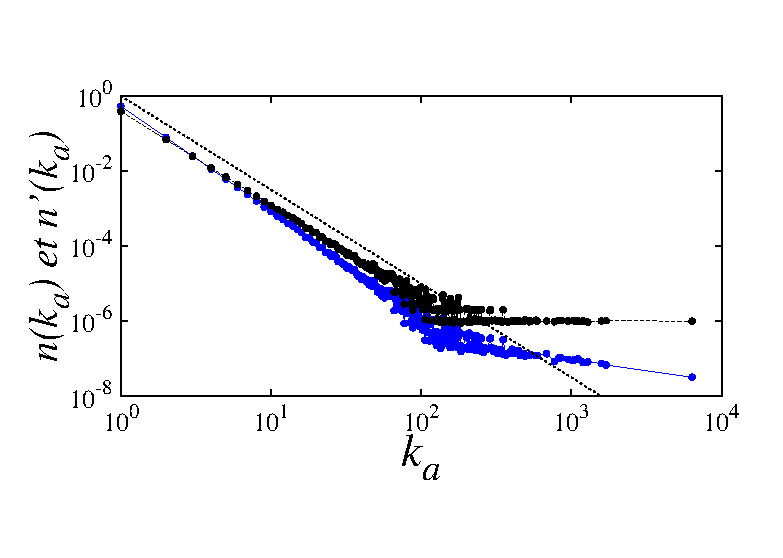
\includegraphics[scale=1.2]{./figures/fig-gama2}
	\caption{La distribution des amas selon deux méthodes différentes pour choisir les noeuds dans le même réseau, la première méthode est aléatoire comme le processus ER (cercles noirs), la deuxièmes est le processus Achlioptas \cite{Achlioptas-al2009} (cercles bleus). La ligne en pointillée  montre  l'exposant  $\beta=2.5$ qu'on trouve lorsque le choix des noeuds est aléatoire. La taille du réseau est $n=10^6$, chaque simulation est une moyenne sur $n$ réalisations. }
	\label{gama-5}
\end{figure}
\subsubsection{Composante géante:}
Dans cette partie nous cherchons une expression de la composante géante plus générale que celle de ER au voisinage du point critique et en fonction des paramètres $\beta$ et $\beta'$.
Nos calculs sont réalisés au voisinage du point critique, qui correspond à $n(k_a)=ck_a^{-\beta}$, puis nous ajoutons des liens au réseau pour permettre l'émergence de la composante géante.
Pour qu'un amas de taille $i$ n'appartienne pas à la composante géante, il ne doit pas être connecté à la composante géante via un autre amas de taille $j$. Cela signifie que: (a) l'amas de taille $i$ n'est pas connecté à l'amas de taille $j$ par un lien, ou (b) l'amas  de taille $i$ est connecté à l'amas de taille $j$ qui n'est pas connecté à la composante géante.\\
Soit $p=\frac{\km}{n-1}$ la probabilité que deux nœuds se connectent, où 
$\km=\frac{2\times\text{(nombre de liens ajoutés)}}{\text{n}}$ est la densité des liens ajoutés par rapport à la taille du réseau.
La probabilité du résultat (a) est $(1-p)^{ij}$, et la probabilité du résultat (b) est $(1-(1-p)^{ij})u$, où $u$ est la probabilité qu'un nœud n'appartienne pas à la composante géante. D'où la probabilité qu'un amas de taille $i$ n'appartienne pas à la composante géante à travers n'importe quel amas de taille $j$ dans le réseau est
\begin{eqnarray}
q_{ij}&=&[(1-p)^{ij}+(1-(1-p)^{ij})u]^{n_an'(j)}\nonumber\\
&\approx&[1-ijp(1-u)]^{n_an'(j)}\nonumber\\
&\approx&e^{-ijp(1-u)n_an'(j)},
\end{eqnarray}
avec $n_a$ est le nombre d'amas et $n_an'(j)=n_ac'j^{-\beta'}$ est le nombre effectif des amas de taille $j$.
D'où la probabilité qu'un amas de taille $i$ n'appartienne pas à la composante géante à travers n'importe quel amas est
\begin{eqnarray}
\pi_{i}&=&\prod_{j=1}^{K}q_{ij}\nonumber\\
&=&e^{-ipn_a(1-u)\sum_{j=1}^{K}jn'(j)},
\end{eqnarray}
où $K_a=n_a^{\frac{1}{\beta-1}}$ est l'amas maximal au voisinage du point critique.\\ D'où $\sum_{j=1}^{K_a}jn'(j)=\kmap$ est la taille moyenne effective des amas. Puisque $\kma$ est la taille moyenne des amas alors $n=n_a\kma$ et sachant que $p=\frac{\km}{n-1}$, on peut écrire
\begin{eqnarray}
\pi_{i}=e^{\frac{-i(1-u)\km\kmap}{\kma}}.
\label{pi}
\end{eqnarray}
La fraction d'amas de taille $i$ qui n'appartiennent pas à la composante géante  est 
\begin{eqnarray}
u_{i}=\frac{n_ain(i)\pi_i}{n},
\label{ui}
\end{eqnarray}
d'où la fraction de nœuds totale qui  n'appartiennent pas  à la composante géante est
\begin{eqnarray}
u=\sum_{i=1}^K u_i.
\end{eqnarray}
Alors la fraction de nœuds qui appartiennent à la composante géante est 
\begin{eqnarray}
S=1-u=1-\sum_{i=1}^{K_a} u_i.
\end{eqnarray}
De l'Eq.~\eqref{pi}, et l'Eq.~\eqref{ui} et sachant que $n=n_a\kma$ et $S=1-u$ on obtient
\begin{eqnarray}
S&=&1-\frac{1}{\kma}\sum_{i=1}^{K_a}in(i)e^{\frac{-iS\km\kmap}{\kma}}\nonumber \\
&=& 1-\frac{1}{\kma}\int_{i=1}^{K_a}in(i)e^{\frac{-iS\km\kmap}{\kma}}di.
\label{s}
\end{eqnarray}
Cette formule est une expression plus générale que celle de modèle ER \cite{Erdos-Renyi1959}. En effet, dans le cas où on ajoute aléatoirement des liens sans corrélations, $\beta=\beta'$, et si au temps initial tout les amas ont la taille $1$, on trouve exactement l'expression de modèle ER, $S=1-e^{-S\km}$.
\begin{figure}[h!]
	\centering
	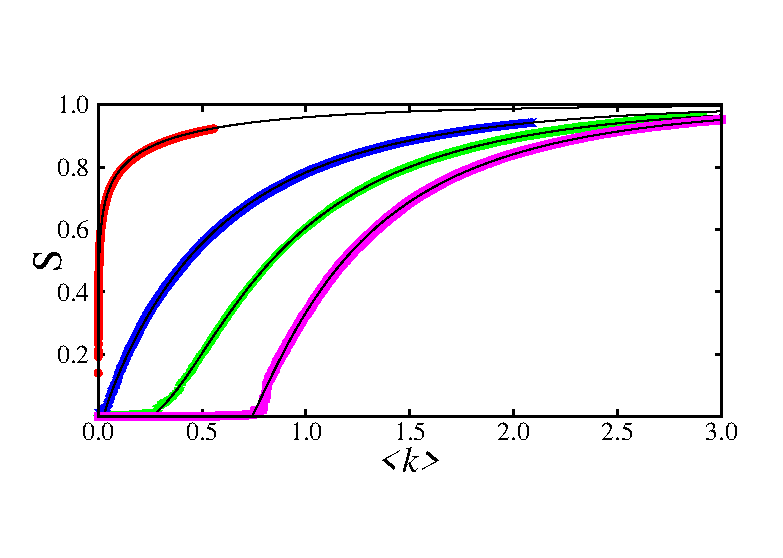
\includegraphics[scale=1.2]{./figures/fig-CG}
	\caption{Fraction de la composante géante $S$ en fonction de la densité des liens $\km$ pour différentes valeurs de $\beta$, les couleurs de gauche à droite représentent les simulations numériques respectivement pour $\beta=2,2.5,3,4$, les lignes noire représentent la solution numérique de l'Eq.~\eqref{s}. Le nombre des nœuds est $n=10^5$.}
	\label{CG}
\end{figure}

\subsubsection{Détermination du point de la transition:}
A partir de Eq.~\eqref{s} et en utilisant la méthode graphique utilisée dans \cite{Newman2010-403} on obtient facilement le point critique ($\km_c$) où la composante géante apparaît, cette méthode s'appuie sur la condition que le point critique $\km$ est donné par 
\begin{equation}
\frac{\partial (1-\frac{1}{\kma}\sum_{i=1}^Kin(i)e^{\frac{-iS\km\kmap}{\kma}})}{\partial S}\Big)_{S=0}=1,
\end{equation}
la solution de cette équation  donne l'expression suivante
\begin{equation}
\km_c=\frac{\kma^2}{\kmaa\kmap},
\end{equation}
dans le cas où il n'y a pas de corrélations $\beta=\beta'$, c'est-à-dire $\kma=\kmap$, on obtient 
\begin{equation}
\km_c=\frac{\kma}{\kmaa}=\frac{1}{\kappa_a},
\label{kc}
\end{equation}
cette expression est différente de celle donnée dans la référence \cite{Cho-al2010} où les auteurs ont trouvé que $\km_c=\frac{1}{\kmaa}$. Cette expression prévoit des valeurs inférieurs à celles prévues par notre équation car $\km_c>1$. La comparaison  de l'Eq.~\eqref{kc} avec les simulations numériques (voir Fig.~\ref{PC}) montre que notre approche est beaucoup plus précise que celle de la référence \cite{Cho-al2010}.\\
\begin{figure}[h!]
	\centering
	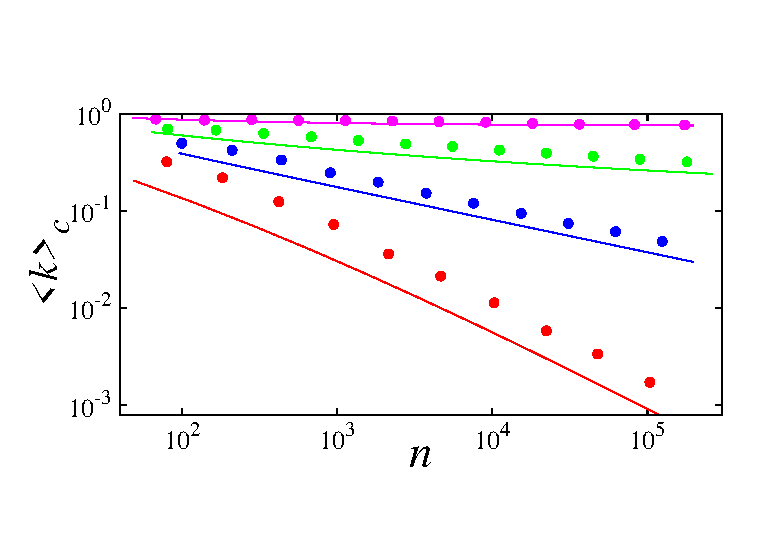
\includegraphics[scale=1.2]{./figures/fig-PC}
	\caption{Estimation de point critique par les simulations numériques (cercles) et par l'Eq.~\eqref{kc} (ligne). Les valeurs de $\beta$ de haut en bas sont respectivement $4,3,2.5,2$. Chaque simulation est moyennée sur $500$ réalisations. }
	\label{PC}
\end{figure}

Il convient de mentionner que la détermination du point de la transition par les simulations n'est pas une opération facile, il est assez compliqué et délicat de trouver le avec une grande précision. Dans nos simulations présentées dans la Fig.~\ref{PC}, nous avons estimé le point de la transition par la détermination du point où la valeur moyenne des petits amas dans le réseau est maximale,  cependant cette estimation est devenue plus précise avec l'augmentation du nombre de nœuds du réseau, car les effets d'échelle diminuent avec la taille. Alors dans la limite thermodynamique l'expression théorique sera souvent exacte. 

\subsubsection{Détermination du type de la transition de phase:}
Pour déterminer le type de la transition de phase on détermine la valeur de $\km$ qui fait que $S$ atteigne une valeur finie $(O(1))$ et on nommé $\Delta k$. Si $\Delta k$ tend vers zéro on dit que la transition est de premier ordre sinon on dit qu'elle est de second ordre\footnote{La condition nécessaire de cette méthode est que le point de la transition doit être tends vers $0$. Autrement dit l'origine du point de la transition doit être au point $\km=0$.} (voir Fig~\ref{fig:continu} et Fig~\ref{fig:discontinu} ). Autrement dit
$\Delta k$ représente la valeur minimale de la densité des liens qu'on doit ajouter au réseau pour faire apparaître la composante géante.  
\\



\begin{figure}
	\centering
	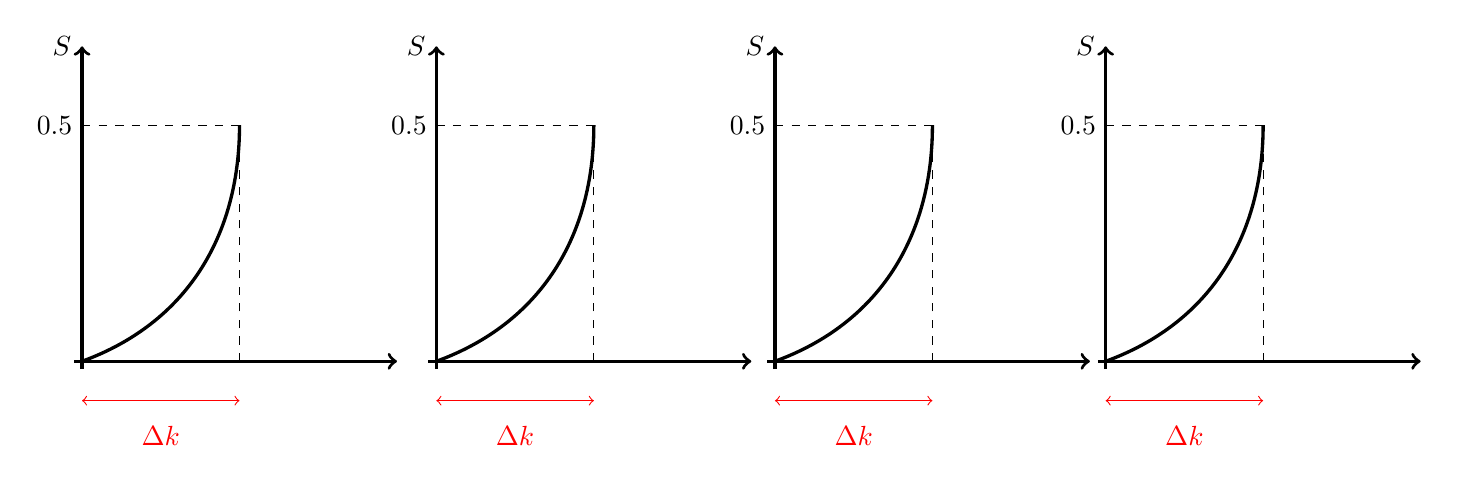
\begin{tikzpicture}
	\begin{scope}[xshift=-1cm,yshift=4cm]
	\draw[very thick] (0,0) node[left] {} to [out=20,in=-90](2,3);
	\draw[->, very thick] (-.1,0) -- (4,0) node[below] {$\km$};
	\draw[->, very thick] (0,-.1) -- (0,4) node[left]{$\text{S}$};
	\draw[dashed] (0,3) node[left] {0.5} to (2,3);
	\draw[dashed] (2,0) node[left] {} to (2,3);
	\draw[<->, red] (0,-0.5) node at (1,-0.95) {$\Delta k$} to (2,-0.5);
	\end{scope}
	\begin{scope}[xshift=3.5cm,yshift=4cm]
	\draw[very thick] (0,0) node[left] {} to [out=20,in=-90](2,3);
	\draw[->, very thick] (-.1,0) -- (4,0) node[below] {$\km$};
	\draw[->, very thick] (0,-.1) -- (0,4) node[left]{$\text{S}$};
	\draw[dashed] (0,3) node[left] {0.5} to (2,3);
	\draw[dashed] (2,0) node[left] {} to (2,3);
	\draw[<->, red] (0,-0.5) node at (1,-0.95) {$\Delta k$} to (2,-0.5);
	\end{scope}
	\begin{scope}[xshift=7.8cm,yshift=4cm]
	\draw[very thick] (0,0) node[left] {} to [out=20,in=-90](2,3);
	\draw[->, very thick] (-.1,0) -- (4,0) node[below] {$\km$};
	\draw[->, very thick] (0,-.1) -- (0,4) node[left]{$\text{S}$};
	\draw[dashed] (0,3) node[left] {0.5} to (2,3);
	\draw[dashed] (2,0) node[left] {} to (2,3);
	\draw[<->, red] (0,-0.5) node at (1,-0.95) {$\Delta k$} to (2,-0.5);
	\end{scope}
	\begin{scope}[xshift=12cm,yshift=4cm]
	\draw[very thick] (0,0) node[left] {} to [out=20,in=-90](2,3);
	\draw[->, very thick] (-.1,0) -- (4,0) node[below] {$\km$};
	\draw[->, very thick] (0,-.1) -- (0,4) node[left]{$\text{S}$};
	\draw[dashed] (0,3) node[left] {0.5} to (2,3);
	\draw[dashed] (2,0) node[left] {} to (2,3);
	\draw[<->, red] (0,-0.5) node at (1,-0.95) {$\Delta k$} to (2,-0.5);
	\end{scope}
	\end{tikzpicture}
	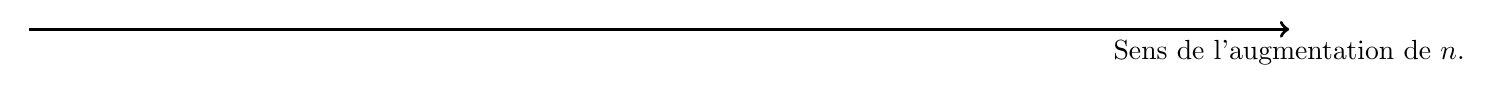
\begin{tikzpicture}
	\draw[->, very thick] (1,0) -- (17,0) node[below] {Sens de l'augmentation de $n$.};
	\end{tikzpicture}
	\caption{Illustration de la variation de $\Delta k$ en fonction de $n$ lorsque la transition est continue. $\Delta k$ est la valeur de $\km$ quand $S=0.5$.} 
	\label{fig:continu}
\end{figure}

\begin{figure}
	\centering
	
		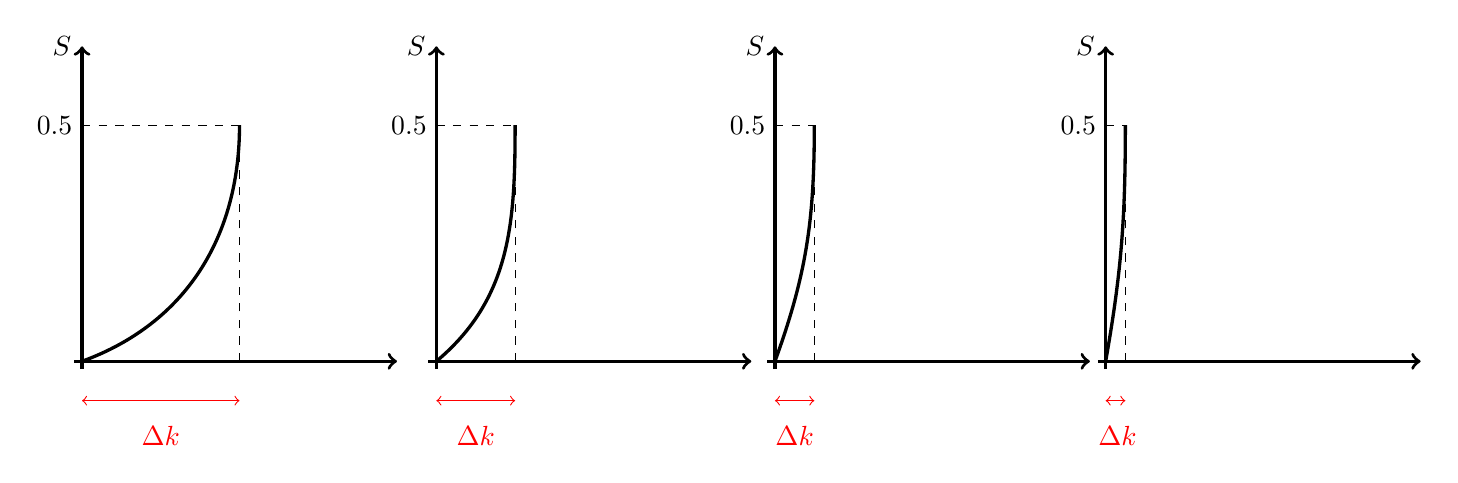
\begin{tikzpicture}
		\begin{scope}[xshift=-1cm,yshift=4cm]
		\draw[very thick] (0,0) node[left] {} to [out=20,in=-90](2,3);
		\draw[->, very thick] (-.1,0) -- (4,0) node[below] {$\km$};
		\draw[->, very thick] (0,-.1) -- (0,4) node[left]{$\text{S}$};
		\draw[dashed] (0,3) node[left] {0.5} to (2,3);
		\draw[dashed] (2,0) node[left] {} to (2,3);
		\draw[<->, red] (0,-0.5) node at (1,-0.95) {$\Delta k$} to (2,-0.5);
		\end{scope}
		\begin{scope}[xshift=3.5cm,yshift=4cm]
		\draw[very thick] (0,0) node[left] {} to [out=40,in=-90](1,3);
		\draw[->, very thick] (-.1,0) -- (4,0) node[below] {$\km$};
		\draw[->, very thick] (0,-.1) -- (0,4) node[left]{$\text{S}$};
		\draw[dashed] (0,3) node[left] {0.5} to (1,3);
		\draw[dashed] (1,0) node[left] {} to (1,3);
		\draw[<->, red] (0,-0.5) node at (0.5,-0.95) {$\Delta k$} to (1,-0.5);
		\end{scope}
		\begin{scope}[xshift=7.8cm,yshift=4cm]
		\draw[very thick] (0,0) node[left] {} to [out=70,in=-90](0.5,3);
		\draw[->, very thick] (-.1,0) -- (4,0) node[below] {$\km$};
		\draw[->, very thick] (0,-.1) -- (0,4) node[left]{$\text{S}$};
		\draw[dashed] (0,3) node[left] {0.5} to (0.5,3);
		\draw[dashed] (0.5,0) node[left] {} to (0.5,3);
		\draw[<->, red] (0,-0.5) node at (0.25,-0.95) {$\Delta k$} to (0.5,-0.5);
		\end{scope}
		\begin{scope}[xshift=12cm,yshift=4cm]
		\draw[very thick] (0,0) node[left] {} to [out=80,in=-90](0.25,3);
		\draw[->, very thick] (-.1,0) -- (4,0) node[below] {$\km$};
		\draw[->, very thick] (0,-.1) -- (0,4) node[left]{$\text{S}$};
		\draw[dashed] (0,3) node[left] {0.5} to (0.25,3);
		\draw[dashed] (0.25,0) node[left] {} to (0.25,3);
		\draw[<->, red] (0,-0.5) node at (0.15,-0.95) {$\Delta k$} to (0.25,-0.5);
		\end{scope}
		\end{tikzpicture}
		
		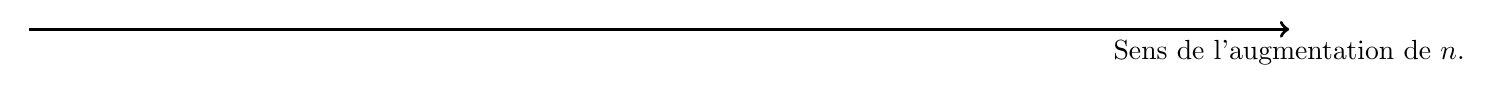
\begin{tikzpicture}
		\draw[->, very thick] (1,0) -- (17,0) node[below] {Sens de l'augmentation de $n$.};
		\end{tikzpicture}
	\caption{Illustration de la variation de $\Delta k$ en fonction de $n$ lorsque la transition est discontinue. $\Delta k$ est la valeur de $\km$ quand $S=0.5$.} 
\label{fig:discontinu}
\end{figure}



A partir de l'Eq.~\eqref{s} et sachant que $n(i)=ci^{\beta}$, on obtient
\begin{equation}
S=1-\frac{c}{\kma}\int_{i=1}^Ki^{1-\beta}e^{\frac{-iS\km\kmap}{\kma}}di
\label{s2},
\end{equation}
l'intégrale dans cette expression n'a pas de solution explicite connue, ce qui rend  impossible l'extraction de $\km$ en fonction de $S$. 
Pour déterminer le type de la transition, on construit la composante géante de la façon suivante:
On commence par un réseau dont la distribution des amas suit une loi de puissance, après et successivement, on ajoute un lien entre les deux plus 
grands amas. Cette construction garantie l'apparition de la composante géante le plus rapidement possible, ce qui implique que si $\Delta k$ est finie (non nulle) alors la transition est sûrement continue, car toute autre construction donnera un $\Delta k$ plus grand. Mathématiquement ceci est traduit par l'expression suivante: 
\begin{equation}
S=\sum_{i=1}^t\frac{k_a(i)}{n}=\int_{1}^{t}\frac{k_a(i)}{n}di,
\label{s3}
\end{equation}
où $t$ représente le temps et également le nombre des liens ajoutés et $k_a(t)$ est $t^{\text{ème}}$ degré maximal, avec $k(1)=K_a$.\\
$k_a(t)$ peut être calculé par l'expression suivante
\begin{equation}
\sum_{i=k_a (t)}^{K_a} n_an(i)=\int_{i=k_a(t)}^{K_a}n_an(i)di=t,
\end{equation}
on obtient
\begin{eqnarray}
k_a(t)&=&\Big(K_a^{1-\beta}+\frac{(\beta-1)t}{cn_a}\Big)^{\frac{1}{1-\beta}}\nonumber\\
&=& \Big(\frac{t+1}{n_a}\Big)^{\frac{1}{1-\beta}} \quad \quad  \text{car} \quad c=\beta-1 \quad \text{et} \quad K_a=n_a^{\frac{1}{\beta-1}} \nonumber\\
&=& \Big(\frac{t}{n_a}\Big)^{\frac{1}{1-\beta}}
\quad \quad  \text{car} \quad t+1\approx t,
\label{kt}
\end{eqnarray}
des Eq.~\eqref{s3} et Eq.~\eqref{kt} on trouve
\begin{equation}
S=\frac{\beta-1}{(\beta-2)\kma}\Big(\big(\frac{t}{n_a}\big)^{\frac{2-\beta}{1-\beta}}-\big(\frac{1}{n_a}\big)^{\frac{2-\beta}{1-\beta}}\Big),
\label{s4}
\end{equation}

sachant que $t=\frac{n\km}{2}$ et $n=n_a\kma$, l'Eq.~\eqref{s4} devient
 $\kma=\frac{\beta-1}{\beta-2}$ et
\begin{equation}
S=\frac{\beta-1}{(\beta-2)\kma}\Big(\Big(\frac{\km \kma}{2}\Big)^{\frac{2-\beta}{1-\beta}}-\big(\frac{1}{n_a}\big)^{\frac{2-\beta}{1-\beta}}\Big),
\label{s5}
\end{equation}
d'où on obtient 
\begin{equation}
\km=\frac{2(\beta-2)}{\beta-1}\Big(\Big(S+\big(\frac{1}{n_a}\big)^{\frac{2-\beta}{1-\beta}}\Big)\frac{\beta-1}{(\beta-2)\kma}\Big)^{\frac{1-\beta}{2-\beta}}.
\end{equation}
Pour $\beta>2$ on a $\kma=\frac{\beta-1}{\beta-2}$, alors pour une valeur de $S$ finie on peut écrire à la limite thermodynamique que $ \km=\frac{2(\beta-2)}{\beta-1}\Big(S\Big)^{\frac{1-\beta}{2-\beta}}$. Sous ces conditions, on peut dire que $\Delta k$ ne peut jamais tendre vers zéro,  ce qui signifie que la transition de phase est sûrement conitnue pour $\beta>2$.\\
On a démontré, donc, qu'il est impossible que la transition de phase soit de premier ordre lorsque l'exposant $\beta>2$  indépendamment de l'exposant effectif $\beta'$, c'est-à-dire indépendamment des corrélations dans le réseau.\\
Lorsque $\beta=2$, l'intégrale de l'Eq.~\eqref{s2} peut se calculer en s'appuyant sur l'approximation suivante  $e^{\frac{-iS\km\kmap}{\kma}}\approx \frac{1}{1+\frac{iS\km\kmap}{\kma}}$, d'où
\begin{eqnarray}
\int_{i=1}^K\frac{i^{-1}}{1+\frac{iS\km\kmap}{\kma}}di&=&\big[\ln(i)-\ln(i\kmaa\km S+\kma)\big]_{i=1}^{i=K}\nonumber\\
&=&\ln(K)-\ln(K\kmaa\km S+\kma)  \quad \quad  \text{car} \quad K\gg 1,
\label{appr}
\end{eqnarray}
en remplaçant l'Eq.~\eqref{appr} dans l'Eq.~\eqref{s2} on obtient 
\begin{equation}
S=1-\frac{c}{\kma}\big(\ln(K)-\ln(K\kmaa\km S+\kma)\big),
\end{equation}
d'où l'expression de $\km$ s'écrit
\begin{equation}
\km=\frac{e^{\frac{c\ln(K)+\kma(S-1)}{c}}-\kma}{K\kmap S},
\end{equation}
sachant que pour $\beta=2$ on a $K_a=n_a$ et $\kma=c\ln(n_a)$, on obtient
\begin{equation}
\km=\frac{n_a^S-c\ln(n_a)}{n_a\kmap S},
\end{equation}
pour $n_a\gg1$ on a $n_a\gg c\ln(n_a)$ et lorsque $S>0$ on peut écrire
\begin{equation}
\km=\frac{n_a^{S-1}}{\kmap S},
\end{equation}
de l'expression ci-dessus il est clair que  $\Delta k$  tend toujours vers $0$ pour toutes les valeurs de $S<1$ et pour n'importe quelle valeur de $\beta'$. Le fait que $\Delta k$ tend vers $0$  signifie que la transition est discontinue à la limite thermodynamique, c'est-à-dire, pour $\beta=2$ il s'agit d'une transition de phase de premier ordre.\\
Nous avons montré, alors, que le type de la transition de phase dépend seulement de la distribution des amas au voisinage du point critique (l'exposant $\beta$), et ne dépend pas des corrélations entre les amas (l'exposant effectif $\beta'$). \\ 
\section{Conclusion}
Dans ce chapitre nous avons étudié quelques propriétés du modèle de percolation dans les réseaux complexes aléatoires. En particulier, on a trouvé l'expression exacte de la composante géante valable pour toutes les distributions de degrés. Ensuite, on a pu établir l'expression qui donne la valeur du point de la transition de phase. Note équation est plus précise que celle dont on dispose actuellement \cite{Cho-al2010}. Finalement on a introduit une nouvelle méthode pour prévoir le type de la transition de phase dans le phénomène de percolation. Contrairement aux autres travaux cités dans la  Section.~\ref{etat-art}, où les auteurs ont essayé de déterminer le type de la transition dans des modèles spécifiques, notre calcul est général et s'appuie sur les paramètres universels de la percolation.  Notre méthode est basée sur deux paramètres, le premier est l'exposant de la distribution des amas au voisinage du point de la transition $\beta$ et le deuxième est l'exposant de la distribution d'amas  effectif $\beta'$ qui est dû aux corrélations dans le réseau. Nous avons trouvé qu'une transition de phase est de premier ordre si $\beta\leq2$, sinon la transition est de second ordre, indépendamment de la valeur de $\beta'$. On en déduit que les corrélations entre les amas au voisinage du point de transition n'ont aucune influence sur le type de la transition de phase.

\let\cleardoublepage\clearpage
